\documentclass{article}
\usepackage[utf8]{inputenc}
\usepackage{graphicx, float}
\usepackage{subfig}

\title{CSP780 Computer Vision: Assignment 2}
\author{SAHIL - 2016UCS0008}
\date{February 24, 2019}

\begin{document}

\maketitle

\section{Introduction}
\large
The given images have been interpolated using the \textbf{bilateral filter}. The following steps are followed in order to do so, independently for each of the colour channels in the image:
\begin{itemize}
    \item An image is interpolated by first copying the pixel values in alternate rows and columns of an image of double its size. The rest of the pixels are zero. 
    \item The zero pixel values are then modified and calculated using the bilateral filter. Assuming it to be the mean of the neighbouring pixels, the bilateral filter is calculated and then convolved with the interpolated image to get the actual value at that location. 
\end{itemize}

\section{Results}

	The original and interpolated image for '1.tif' are shown below. \\
	The quality of the image is maintained and the edges are preserved as we have used a bilateral filter for interpolation. 
	
	\begin{figure}[H]
		\centering
		\subfloat[1.tif original]{{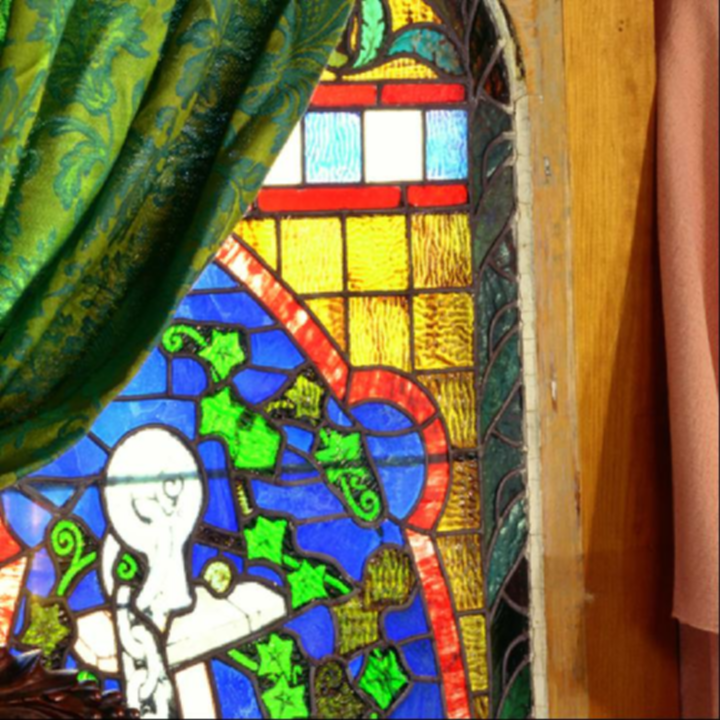
\includegraphics[width=2.5cm, height=2.5cm]{./1.png}}}
		\qquad
		\subfloat[1.tif interpolated]{{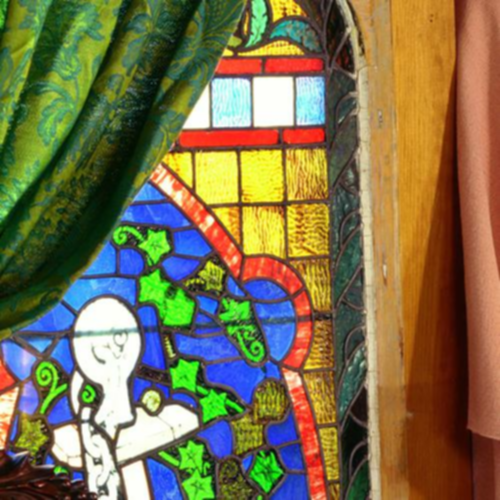
\includegraphics[width=5cm, height=5cm]{./1_interpolated.png} }}
		\caption{Applying interpolation on 1.tif}
	\end{figure}
	
	For measuring PSNR scores, the reference used is the CV2's inbuilt resize function which uses bilinear interpolation. 
	 
	\begin{figure}[H]
		\centering
		\vspace{0pt}
		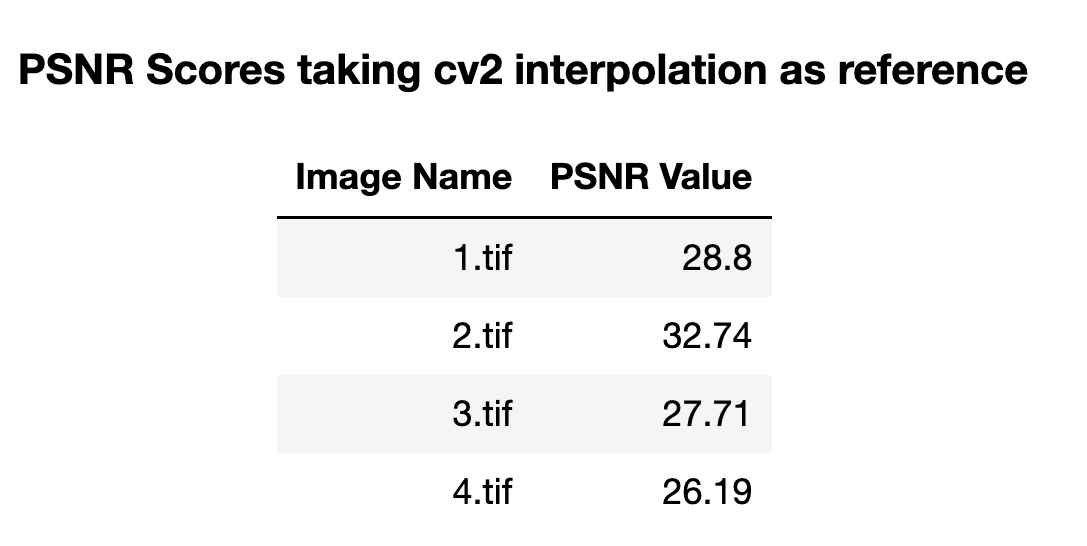
\includegraphics[width=400pt, height = 150pt, keepaspectratio]{./psnr_scores.png}
		\caption{Table showing the PSNR scores}
	\end{figure}
	
\end{document}
